%% This is an example first chapter.  You should put chapter/appendix that you
%% write into a separate file, and add a line \include{yourfilename} to
%% main.tex, where `yourfilename.tex' is the name of the chapter/appendix file.
%% You can process specific files by typing their names in at the 
%% \files=
%% prompt when you run the file main.tex through LaTeX.
\chapter{The CMS experiment}
The major goal of the CMS detector~\cite{Chatrchyan:2008aa} is to elucidate the EWSB through the discovery of the Higgs boson. However CMS is a general purpose detector enabling to perform precision SM measurements as well BSM physics searches at the $\TeV$ scale. The detector requirements, driven by the physics program, include good reconstruction and momentum resolution of charged particles, good electromagnetic energy resolution, as well as good di-jet mass and missing energy resolutions. The large number of charged particles per interactions and the additional pileup interactions require a high granularity detector to be able to reconstruct all the individual charged particles.  Furthermore, a bunch spacing of $25$ ns requires a detector with good time resolution to be able to resolve the individual bunch crossings.  

The overall layout of the CMS detector is shown in Figure~\ref{fig:cms}. The detector is composed of several sub-detector layers with a length of $22$ m and a diameter of $15$ m. It has a cylindrical geometry with concentric barrel shaped detectors in the central region and disc shaped detectors in the forward region. The main feature of the CMS detector is a $3.8$ Tesla superconducting solenoid magnet that provides a large bending power to the charged particles. The length of the solenoid is $13$ m and the inner diameter is $6$ m. The inner tracking detectors, electromagnetic, and hadron calorimeters are located inside the solenoid. The muon detectors are embedded in the steel flux-return yoke of the magnet providing a sufficient magnetic field for a large bending power of the muons inside the muon detectors. The total weight of the CMS detector is $12500$ tonnes.  

\begin{figure}[h]
\centering
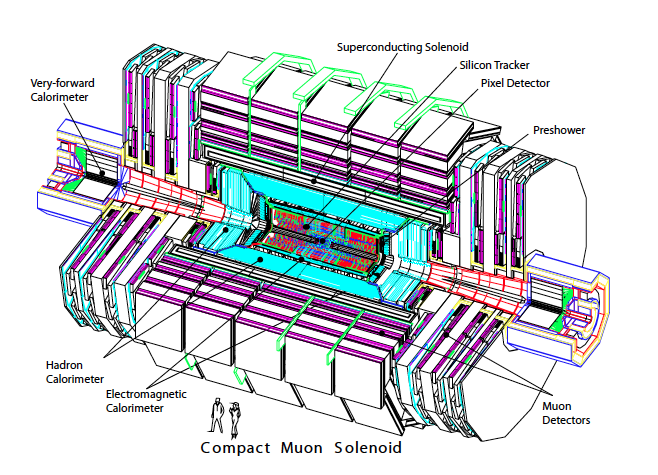
\includegraphics[width=1.0\columnwidth]{figures_chapter3/cms_detector}
\caption{A cutaway diagram of the CMS detector. The labels identify the different sub-detectors and the solenoid.}
\label{fig:cms}
\end{figure}

CMS uses the right-handed coordinate system. The origin is centered at the nominal collision point, x-axis is in the horizontal plane pointing towards the centre of the LHC tunnel, y-axis points vertically upwards, and the z-axis points along the beam direction toward the Jura mountains. It is convenient to employ the spherical coordinate system. The polar angle  $\theta$ is measured with respect to the positive z-axis and the azimuthal angle $\phi$ is measured from the positive x-axis in the x-y coordinate plane. The pseudorapidity is defined as $\eta = -\ln \tan(\frac{\theta}{2})$.  A useful consequence of this definition is that the difference between the pseudorapidities of two particles is Lorentz invariant with respect to a boost in the beam direction. The separation of two particles is defined by $\Delta R =\sqrt(\Delta \phi^2 + \Delta \eta^2)$. The momentum and energy transverse to the beam direction are denoted $p_{T}$ and $E_{T}$ respectively. The imbalance of the measured transverse energy is defined as a missing energy and denoted by $E_{T}^{miss}$.     

\section{Inner tracking detectors}

The inner tracking system~\cite{Karim�ki:368412,addendum} surrounds the interaction point and has a length of $5.8$ m and a diameter of $2.5$ m. The goal of the inner tracking system is to make a precise and efficient measurement of the trajectories of charged particles as well as their momentum. In addition a precise reconstruction of secondary vertices is needed for the identification of heavy flavor particle decays. Tau lepton decays are identified by looking for one-prong and three-prong topologies in the inner tracker. A homogenous magnetic field of $3.8$ Tesla over the full volume of the tracker is provided by the CMS solenoid. 

There are $\mathcal{O}(1000)$ particles emerging from the interaction region at the nominal LHC luminosity for every $25$ ns bunch crossing. Therefore a high granular, fast, and radiation hard detector is required. On the other hand this implies a large power density of electronics and the corresponding cabling and cooling systems which increases the amount of material thereby enhancing the multiple scattering, photon conversions, and bremsstrahlung.    Silicon technology was chosen given the above considerations. Figure~\ref{fig:tracker} shows a schematic view of the inner tracking system in $r-z$ plane. The inner tracking detector covers a pseudorapidity range of up to $|\eta|=2.5$ and provides an average of $13-17$ measurements per charged particle depending on the $\eta$ region.

\begin{figure}[h]
\centering
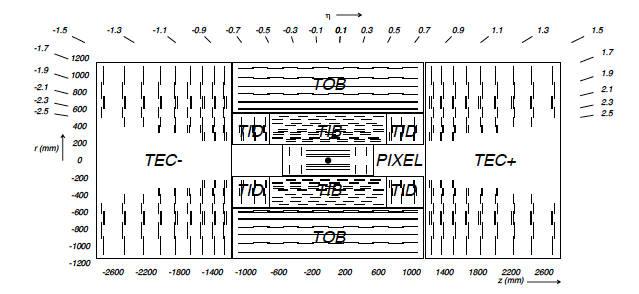
\includegraphics[width=1.0\columnwidth]{figures_chapter3/tracker_layout}
\caption{A schematic view of the CMS tracking system. Silicon pixel and strip detectors are shown. The double lines show back-to-back modules that deliver stereo hits.}
\label{fig:tracker}
\end{figure}

A pixelated detector has to be used close to the interaction region to keep the occupancy levels to less than $1\%$. The tracking system consists of three barrel layers and two endcap disks. The barrel layers are located at radii of $4.4$, $7.3$, and $10.2$ cm with a length of $53$ cm. The endcap pixel layers are located at $z=\pm 34.5$ and $z=\pm46.5$ cm covering approximately $6$ to $15$ cm in the radial direction. The pixel detector consists of $66$ million pixel elements covering a surface area of approximately of $1$ m$^2$. The pixel element size is $100\times150$ $\mu$m$^2$ providing a similar track resolution in both $r-\phi$ and $r-z$ directions. Each pixel is a $p-n$ semiconductor junction. When a charged particle passes through the depletion region of the junction an electron-hole pairs are created and subsequently collected by the readout electronics. The Lorentz drift in the CMS magnetic field leads to a charge spreading of the collected signal charge between adjacent pixels. Using an analog pulse height read out the charge sharing allows to reduce a single hit spatial resolution to $15-20$ $\mu$m.  

The outer tracker is occupied by a silicon strip tracker allowing two-dimensional measurements. Majority of the strips are oriented perpendicular to the $\phi$ direction, parallel to the beam direction in the barrel region and aligned radially in the endcap region. The tracker Inner Barrel (TIB) is located in the barrel region and extends from $20$ cm to $55$ cm in the radial direction. There are $6$ additional layers with an outer radius of $116$ cm composing the Tracker Outer Barrel (TOB) and extending in $|z|$ to $118$ cm. The Tracker Disk (TID) consists of $3$ layers located from $|z|$ of $80$ to $90$ cm. The Tracker EndCap (TEC) has nine layers and covers the region between $|z|$ of  $124$ and $282$ cm. These radial strips provide up to  $9$ $\phi$ measurements for each trajectory. The silicon strip tracker has a total of $9.3$ million strips and covers a surface area of $198$ m$^2$. The strip pitch varies between $80$ and $184$ $\mu$m depending on the region of interest. In addition, there is a second strip module mounted back-to-back with a stereo angle of $100$ mrad in the first layers. This allows a measurement of the $z$ and $r$ coordinates in the barrel and disks respectively. The corresponding resolution in z coordinate is $230$ to $530$ $\mu$m in TIB and TOB respectively.  

\section{Electromagnetic calorimeter}

The goal of the CMS electromagnetic calorimeter (ECAL)~\cite{ecal,CMS:2002xia} is to measure the energy of electrons and photons. ECAL is a homogeneous and hermetic calorimeter made of $61200$ lead tungstate (PbWO$_4$) crystals in the central barrel region (EB) and $14648$ crystals in the endcap region (EE). A homogeneous calorimeter was chosen to achieve the best energy resolution as one of the driving criteria was the precise measurement of the decay of the Higgs boson to two photons. Incident photons and electrons initiate an electromagnetic shower in the PBWO$_4$ crystals. The particles in the shower produce blue-green scintillation light as they excite the crystals and the scintillation light is measured by the photodetectors to determine the energy deposited in the crystals.   

Lead tungstate high density ($8.3$ g/cm$^3$) crystals were chosen to satisfy the challenging operational requirements at the LHC. The scintillation decay time of these crystals is of the same order as the LHC bunch crossing with $80\%$ of the light emitted in $25$ ns. A short radiation length of $X_{0}=0.89$ cm and a small Moliere radius of $2.2$ cm allows to have a fine granular and a compact calorimeter while still containing the electromagnetic showers in longitudinal and transverse directions. The crystals are radiation hard but there is a transparency loss under exposure to an ionizing radiation with a dynamical recovery when there are no collisions. The transparency loss is corrected with a dedicated laser monitoring system. 

\begin{figure}[h]
\centering
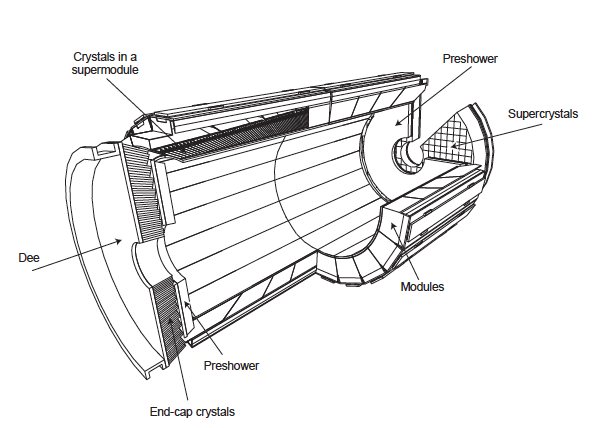
\includegraphics[width=1.0\columnwidth]{figures_chapter3/cms_ecal}
\caption{The layout of the CMS electromagnetic calorimeter. The barrel and endcap calorimeters are shown. The pre-shower detector sits in front of the endcap ecal.}
\label{fig:ecal}
\end{figure}

Figure~\ref{fig:ecal} shows the layout of the ECAL. The $61200$ crystals in EB are arranged in a $170\times360$ $\eta-\phi$ grid with a coverage up to $|\eta|=1.479$ in presudorapidity. The crystal front face cross section is approximately $0.0174\times0.0174$ in $\eta-\phi$ ($22-22$ mm$^2$) and $26-26$ mm$^2$ at the rear face. The increase in cross sectional area of the rear face is consistent with the small Moliere radius allowing to contain the transverse development of the electromagnetic shower within few crystals with respect to the central crystal. Each crystal has a length of $230$ mm corresponding to $25.8$ radiation lengths allowing to contain the longitudinal shower development with negligible levels of leakage. The crystals make an angle of $3$ degrees with respect to the particle trajectories incident from the interaction vertex to avoid cracks aligned with the trajectories. Two avalanche photodiodes (APDs) with an active are of $5\times5$ mm$^2$ are connected to the back of the crystals to convert the scintillation light to photo-electrons.   

The $14648$ crystals in EE are arranged in an $x-y$ grid with a front face cross section of $28.62\times28.62$ mm$^2$ and a rear face cross section of $30\times30$ mm$^2$. The length of the crystals is $220$ mm corresponding to $24.7$ radiation lengths. Vacuum phototriodes (VPTs) with an active area of approximately  $280$ mm$^2$, allowing large surface coverage, are used as photodetectors. An anode of very fine copper mesh allows to operate these devices in the $3.8$ Tesla magnetic field with only slight lose in gain. The EE extends the ECAL coverage from $|\eta|=1.479$ to $|\eta|=3.0$. A sampling preshower detector sits in front of the EE allowing the identification of neutral pions from $|\eta|=1.7$ to $|\eta|=2.6$. Two alternating layers of passive led and active silicon layers form a sampling calorimeter with approximately $3$ radiation lengths of the absorber material.  

The energy resolution of the ECAL can be parameterized as
\begin{equation} \label{eq:ecal_resol}
\frac{\sigma}{E} = \frac{S}{\sqrt{E}} \oplus  \frac{N}{E} \oplus C,
\end{equation}
where $E$ is the energy of the incident particle, $S$ is the stochastic term, $N$ is the noise term, and $C$ is the constant term. The longitudinal shower leakage is assumed to be negligible in (\ref{eq:ecal_resol}). Event-to-event fluctuations in the lateral shower containment and the photo-statistics of $2.1\%$ contribute to the stochastic term. The noise term is mostly due to the electronic and digitization noise while the constant term comes from intercalibration errors and a non-uniform light collection. Typical values found at an electron test beam are $S=0.029~\GeV^{\frac{1}{2}}$, $N=0.12~\GeV$, and $C=0.003$.    

\section{Hadron calorimeter}

The goal of the CMS hadron calorimeter (HCAL)~\cite{hcal} is to measure the energy of charged and neutral hadrons. This is particularly important for the measurement of hadronic jets and transverse missing energy. Figure~\ref{fig:hcal} shows the layout of the hadron calorimeter components in the $r-z$ coordinate plane. The HCAL barrel calorimeter (HB) sits behind the ECAL between a radius of $r=1.77$ m and the inner extend of the magnetic coil ($r=2.95$ m). The HB is a sampling calorimeter extending to $|\eta|=1.3$ in pseudorapidity with $0.087\times0.087$ segmentation in $\eta-\phi$. The first layer of the absorbing material is a $40$ mm thick steel plate followed by eight $50.5$ mm thick brass plates with a last layer of $75$ mm thick steel plate. The chemical composition of the non-magnetic brass is $70\%$ Cu and $30\%$ Zn with a radiation length of $1.49$ cm. Thus the total absorber thickness is $5.8$ interaction lengths ($\lambda_{I}$) at $\eta=0$ and increasing to $10.6$ $\lambda_{I} $ at $|\eta|=1.3$. It has to be noted that the ECAL in front of HB adds about $1.1$ $\lambda_{I}$  of additional material.      

\begin{figure}[h]
\centering
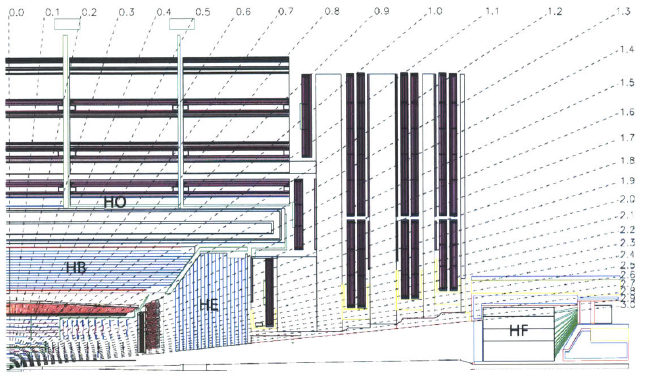
\includegraphics[width=1.0\columnwidth]{figures_chapter3/cms_hcal}
\caption{The layout of the CMS detector in the $r-z$ coordinate plane showing the location of the hadron barrel, endcap, outer, and forward calorimeters. The dashed lines show the extend of the coverage in pseudorapidity.}
\label{fig:hcal}
\end{figure}      

Plastic scintillators  ($3.7$ mm thick) are used for the active layers using a tile and wavelength shifting fiber setup to bring out the light. The first and last layers of the scintillators are $9$ mm thick where the latter serves to correct for the late developing hardon showers leaking out the back of the HB while the former serves to sample the hardon showers developed in the inert material between the EB and HB. Clear fibers are spliced onto the wavelength shifting fibers which are connected to optical fibers that take the light to an optical decoding unit (ODU). The role of the ODU is to arrange the fibers into read-out towers and bring the light to the hybrid photodiodes (HPDs)~\cite{Cushman2000289}. The central component of the HPD is a photocathode held at a high voltage of $-8$ kV from a pixelated silicon photodiode.  The accelerated photo-electon from the cathode produces an ionization in the diode ($3.3$ mm away) with an overall gain of about $2000$. 

 The hadron endcap (HE) extends the pseudorapidity coverage to $|\eta|=3.0$ providing about $10$ $\lambda_{I}$ interaction lengths (including the ECAL crystals). The granularity of the HE is $0.087\times0.087$ in $\eta-\phi$ for $|\eta|<1.6$ and $0.17\times0.17$ for $|\eta|\geq 1.6$. The EB and HB absorbing power does not provide sufficient containment of the hadronic showers. An additional outer calorimeter (HO) that utilizes the solenoid  as an absorbing material is placed in the iron yoke (radial distance of $4.1$ m) that returns the solenoid magnetic field. There is an additional sensitive layer at a radial distance of $3.8$ m at $\eta=0$ as the HB has minimal absorbing length there. The total absorber thickness is increased to a maximum of $11.8$ $\lambda_{I}$ through the inclusion of the HO.
 
The forward calorimeter (HF) extends the pseudorapidity coverage to $|\eta|=5.2$. The HF is also responsible for the measurement of electromagnetic energy since the coverage of ECAL extends only to $|\eta|=3.0$.   
The particle flux in this region is extremely high; presenting a hostile conditions for the detector and requiring a radiation hard active material. Steel absorber layers and scintillating quartz fibers are used as the passive and active materials respectively. The absorption depth is approximately $10$ $\lambda_{I}$. Cherenkov light is generated in the quartz fibers when the charged shower particles are above the Cherenkov threshold. Thus the HF is mostly sensitive to the electromagnetic component of the showers. The HF has a longitudinal segmentation of two segments that allows to distinguish between incident electrons/photons and hadrons. This is accomplished by having two sets of fibers where one set only starts at a depth of $22$ cm from the front end of the detector. The transverse segmentation is $0.175\times0.175$ in $\eta-\phi$. The Cherenkov light is measured by a standard bialkaline  high gain photomultiplier tube with a borosilicate glass in the fringe magnetic field of the solenoid. 

\subsection{HCAL upgrades during the long shutdown $1$ and $2$}

There is a comprehensive program to upgrade the HCAL detectors to take advantage of technologies that have become available since the original design of the detector~\cite{Mans:1481837}. The Phase $1$ upgrade of the CMS HCAL is designed to improve the performance of the calorimeters at high luminosities with mean number of about $50$ pileup events expected at the LHC. The HPDs in the HB and HE will be replaced by silicon photomultiplier (SIPM) devices while the single-channel phototubes in the HF will be replaced by multi-anode phototubes operated in a dual-anode configuration to reject spurious signals  present in the single-channel phototubes. The readout detectors of all the calorimeter detectors will be replaced as well. 

\begin{figure}[h]
\centering
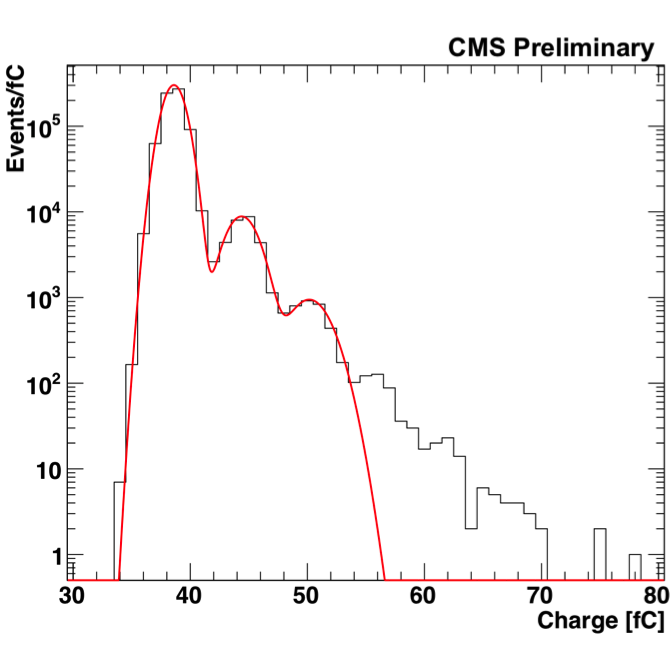
\includegraphics[width=0.6\columnwidth]{figures_chapter3/sipm2.png}
\caption{Charge distribution in a SIPM for events with no incident photons~\cite{CMS-DP-2014-013}. The first peak is due to the leakage current while the subsequent peaks show the thermal avalanches of individual pixels. The red curve is a fit to the charge distribution.}
\label{fig:sipm}
\end{figure}

The Phase $1$ upgrade program will be carried out during the long shutdown $2$ (LS2) starting in $2018$. However, the HPDs in the HO calorimeter were already replaced by SIPMs during LS1. SIPMs are pixel arrays of avalanche photodiodes each operating in Geiger mode. Adding the signal of all the pixels together gives a measurement of the number of incident photons. SIPMs are compact devices that operate at about $2$ orders of magnitude lower voltages compared to the HPDs. The gain is similar to that of photomultipliers but the quantum efficiencies are a factor of $2$ higher compared to the HPDs. In addition, the SIPMs are not affected by magnetic fields of up to $4$ Tesla while about $10\%$ of the HPDs experience rapid breakdown at lower magnetic fields affecting the HO calorimeter in the fringe fields outside of the solenoid. 

SIPMs have an order of magnitude higher signal to noise ratios compared to the HPDs. The low signal to noise ratio is evident in Figure~\ref{fig:sipm} showing the thermal avalanches of individual pixels. The performance of the SIPM devices allows to increase the depth segmentation of the HB and HE calorimeters. The current depth segmentation is summarized in Figure~\ref{fig:depth}. The current HB calorimeter has a single longitudinal readout for most of the towers.  
 
\begin{figure}[h]
\centering
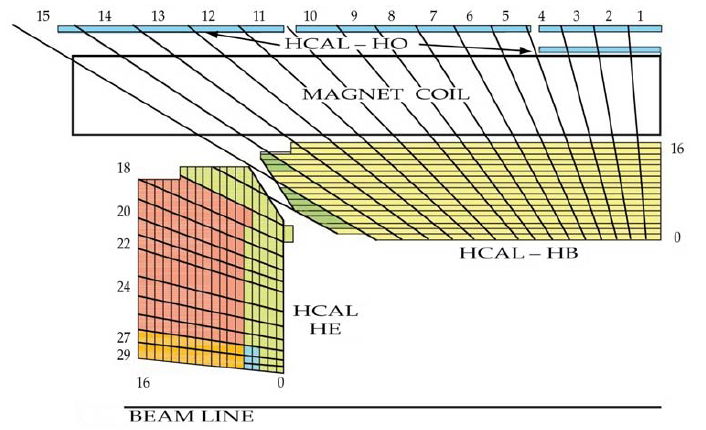
\includegraphics[width=1.0\columnwidth]{figures_chapter3/depth}
\caption{The current HCAL segmentation in the $r-z$ coordinate plane. The grouping of colors represents the optical grouping of the scintillator layers into different readouts.}
\label{fig:depth}
\end{figure} 
 
\section{Muon Detectors}

The goal of the CMS muon detectors~\cite{cms_muon} is threefold: muon triggering, identification, and the momentum measurement. Muons are minimum ionizing particles and there is little energy loss due to bremsstrahlung as muons have about $200$ times larger mass than electrons. Muons are detected in gas-ionization detectors embedded in the the steel return yoke outside of the solenoid. An appearance of a charged particle in the muon detectors is a strong indication of a muon particle as the charged hadrons, electrons, and photons are effectively stopped by the ECAL and HCAL.   

The layout of the CMS muon system is shown in Figure~\ref{fig:muon_layout} providing a pseudorapidity overage to $|\eta|=2.4$. Drift tube (DT) chambers with rectangular drift cells are used in the central barrel region with a pseudorapidity coverage to $|\eta|=1.2$. There are $4$ stations cylindrically interspersed in the layers of the flux return plates where the first $3$ stations contain $8$ chambers measuring the muon coordinate in the $r-\phi$ plane and $4$ chambers providing a measurement in the $z$ direction along the beam-line. The last station does not have the $z$ measurement plates. The gas used in the drift cells is a mixture of argon and carbon dioxide. The maximum drift time is $380$ ns in this mixture corresponding to a drift length of $21$ mm.  

\begin{figure}[h]
\centering
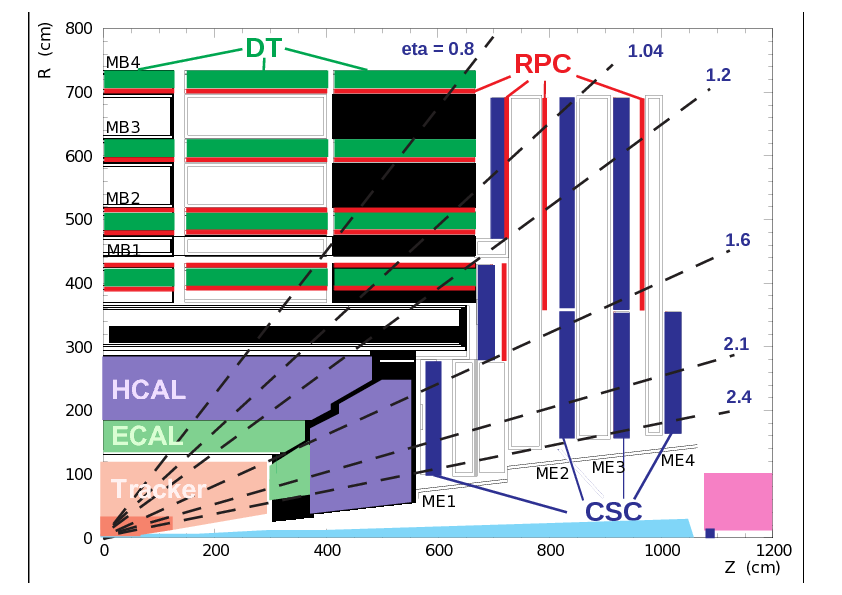
\includegraphics[width=1.0\columnwidth]{figures_chapter3/cms_muon_layout}
\caption{The layout of the CMS detector in the $r-z$ coordinate plane showing the location of the four DT chambers in the barrel (MB1-MB4) and the four CSC chambers in the endcap (ME1-ME4). The RPC stations are shown in red~\cite{Chatrchyan:2012xi}. The dashed lines show the extend of the coverage in the pseudorapidity.}
\label{fig:muon_layout}
\end{figure}   

Cathode strip chambers (CSCs) are used in the endcap region, where the muon rates and background levels are higher, with a pseudorapidity coverage from $|\eta|=0.9$ to $|\eta|=2.4$. The CSCs are radiation resistant and have a fast response time and fine segmentation. There are $4$ stations with chambers positioned perpendicular to the beam line with the cathode strips of each chamber running radially outward to provide measurements in the $r-\phi$ plane. The anode wires are also read out. They run perpendicular to the strips and provide measurements in $\eta$. 

A dedicated trigger system consisting of resistive plate chambers (RPCs) is added covering up to $|\eta|=1.6$ in pseudorapidity. The RPCs are double-gap chambers that operate in avalanche mode. The response is very fast with a time resolution of about $1$ ns. They serve as an independent muon trigger system that can identify the correct bunch crossing time at the LHC nominal instantaneous luminosity. The position resolution of the RPCs is  poorer than the DTs and CSCs. 

\begin{figure}[h]
\centering
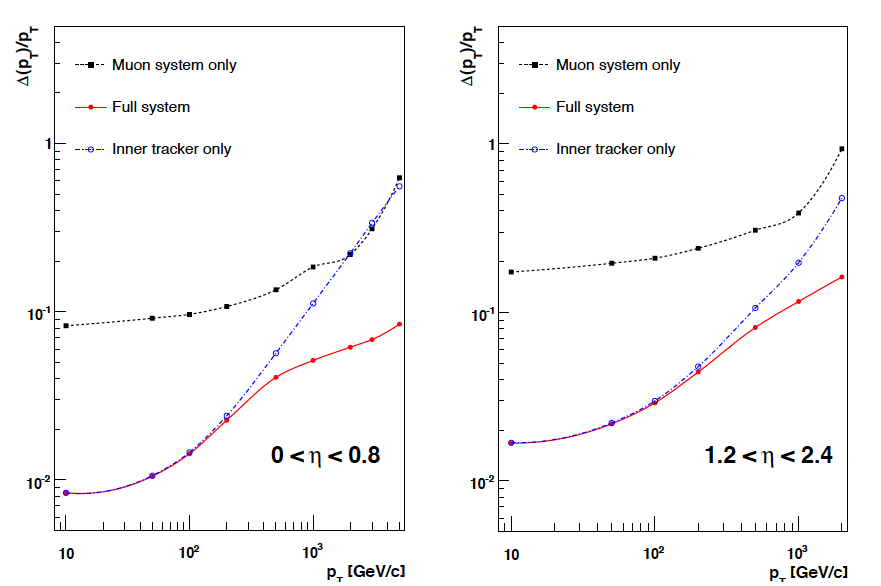
\includegraphics[width=1.0\columnwidth]{figures_chapter3/momentum_resolution}
\caption{The expected muon transverse momentum resolution as a function of the transverse momentum for $|\eta|<0.8$ (left panel) and $1.2<|\eta|<2.4$ (right panel)~\cite{Chatrchyan:2008aa}. The performance for the muon system only (black), the inner tracker only (blue), and the full system (red) is shown.}
\label{fig:muon_resolution}
\end{figure}  

Figure~\ref{fig:muon_resolution} shows the expected muon transverse momentum resolution using the standalone muon system (black) and the inner tracking system (blue). A muon resolution of about $9\%$ for muon transverse momenta up to $200~\GeV$ is achieved. Multiple-scattering in the detector material before the first muon station limits the resolution achieved by the standalone muon system. An order of magnitude improvement in resolution is achieved using the inner tracker information in a global momentum fit, as described in the next chapter (the red curves in Figure~\ref{fig:muon_resolution}).     

\section{Triggering and Data Acquisition}

The design $25$ ns bunch spacing at the LHC translates to a bunch crossing rate of $40$ MHz. This results in a total inelastic collision rate of order of $1$ GHz taking the additional inelastic proton-proton interactions per bunch crossing into account. A drastic rate reduction has to be achieved as it is impossible to store and process the resulting large amount of data. This is achieved by the triggering system. The triggering of the events in the CMS is achieved in two steps designated as Level One Trigger (L1)~\cite{Bayatyan:706847,Khachatryan:2016bia} and High-Level Trigger (HLT)~\cite{Khachatryan:2016bia,Cittolin:578006,Adam:2005zf}. The L1 trigger consists of a custom designed and largely programmable electronics while the HLT is a software system consisting of a farm of about one thousand commercial processors having a few thousand CPU cores. The L1 trigger takes the decision to either reject or accept the event for further evaluation by the HLT. Thus the events are readout and fully assembled only for the events that pass the L1 trigger. The readiness of the sub-detectors and the data acquisition (DAQ) system are considered in the L1 decision through the Timing, Trigger, and Control (TTC) system~\cite{Varela:687458}. Finally the events are either discarded or passed to the offline computing system for storage and reconstruction depending on the HLT decision. The nominal output rate of the L1 trigger is $100$ kHz limited by the CMS readout electronic speed.  The HLT selects an average rate of $400$ Hz for storage and processing. However HLT accept rates of up to several kHz are possible if the data is not processed promptly. An extra $300-400$ Hz data was collected through special "parked" data stream~\cite{CMS-DP-2012-022} during the $2012$ data taking period and reconstructed only at the end of the run. The overall output rate of the L1 trigger and HLT can also be adjusted by applying a pre-scale on the number of events that satisfy the selection criteria of specific algorithms. 

\begin{figure}[h]
\centering
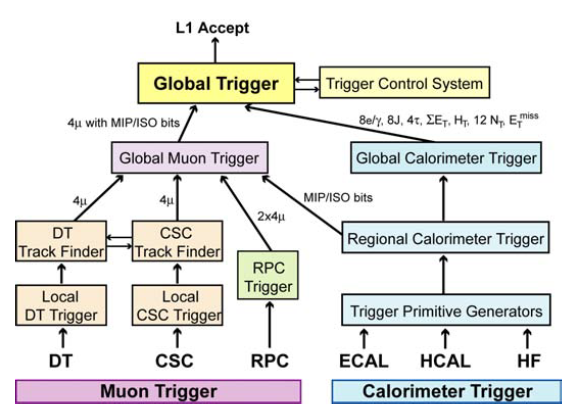
\includegraphics[width=0.8\columnwidth]{figures_chapter3/l1trig}
\caption{Level-1 trigger architecture showing the components of the trigger~\cite{Chatrchyan:2008aa} .}
\label{fig:l1trig}
\end{figure}  

The L1 trigger uses coarsely segmented data from the calorimeters and the muon system. The full detector information is retained in the pipelined memory buffers of the front-end read-out electronics pending the L1 trigger decision. It has to be noted that no information from the inner tracking system is used in the L1 trigger as the number of channels and the speed of the readout electronics of the inner tracking detectors is currently prohibitive. The L1 hardware  is implemented in combination of Field Programmable Gate Arrays (FPGAs) and Application Specific Integrated Circuits (ASICs). A programmable memory lookup table (LUT) is also used where density and radiation requirements are important. The allowed latency is $3.2$ $\mu$s. Figure~\ref{fig:l1trig} shows the L1 trigger architecture and the information flow toward the L1 decision. The L1 trigger objects consist of clusters of the ECAL and HCAL deposits (photons/electrons, hadrons), muons, and global event information such as the summed transverse energy or the missing transverse energy. 

The HLT has access to the complete read-out data including the hit patterns from the inner tracking detector. Thus better position and momentum resolutions can be used compared to the L1 trigger objects. The HLT uses identical software framework to the one used in the offline processing. However optimized algorithms and configurations are used to manage the input rate of $100$ kHz. For example, reconstruction of the tracks in the inner tracking system is only performed after other selection criteria based on the calorimeter and muon detector information to reduce the CPU usage. In addition, the data is reconstructed in the regions of interest, defined by the L1 trigger information, to further reduce the processing time.  The output rate of the HLT is limited by event sizes and the capacity of the downstream systems to process the events.   

\section{Detector Simulation}

A full detector simulation is performed using Geant $4$~\cite{Agostinelli:2002hh,Allison:2006ve}. The simulation includes the propagation of the final state particles in the CMS magnetic field as well as the passage of the particles in the passive and active elements of the detector. The readout electronics are simulated including the effects of the noise. The output of the simulation has the same format as the collision data. Thus, a complete simulation is obtained starting from the generated events described in section 1.3, and adding the simulated detector response. The effects of the pileup interactions are modeled by including additional inelastic proton-proton collisions in the event according to a distribution of pileup events expected in data. The simulated events are then reconstructed using the same reconstruction software used for the collision data events. 
